\documentclass{sig-alternate}
\usepackage{txfonts}
\usepackage{ifpdf}
\usepackage{amsmath}
\usepackage{mathrsfs}
\usepackage{amsfonts}
\usepackage{subfigure}
\usepackage{graphicx}
\usepackage{latexsym}
\usepackage{multirow}
\usepackage{microtype}
\usepackage{algorithm}
\usepackage{paralist}
\usepackage[sort]{cite}
\usepackage[pdfborder={0 0 0},plainpages,pdfpagelabels=false]{hyperref}

\setlength{\paperheight}{11in}
\setlength{\paperwidth}{8.5in}

\newtheorem{theorem}{Theorem}
\newtheorem{proposition}[theorem]{Proposition}
\newtheorem{claim}[theorem]{Claim}
\newtheorem{lem}[theorem]{Lemma}
\newtheorem{terminology}[theorem]{Terminology}
\newtheorem{corollary}[theorem]{Corollary}
\newtheorem{observation}[theorem]{Observation}
\newtheorem{problem}[theorem]{Problem}


\newtheorem{defi}[theorem]{Definition}
\newtheorem{exa}[theorem]{Example}

% QED symbol at the end of definitions and examples
\newif\ifqedwritten
\newenvironment{definition}[1][]{\begin{defi}[#1]\upshape\qedwrittenfalse}{\qedhere\end{defi}}
\newenvironment{example}{\begin{exa}\upshape\qedwrittenfalse}{\qedhere\end{exa}}
\newcommand{\qedhere}{\ifqedwritten\else\ifmmode\tag*{\qed}\else\hfill\qed\fi\global\qedwrittentrue\fi}

\newcommand{\topk}{\mbox{top-$k$}}
\newcommand{\Topk}{\mbox{Top-$k$}}
\newcommand{\topkm}{\mbox{top-$k$,$m$}}
\newcommand{\Topkm}{\mbox{Top-$k$,$m$}}

\renewcommand{\leq}{\leqslant}
\renewcommand{\geq}{\geqslant}

% More tolerant setting for floats -- more compactness
\renewcommand\floatpagefraction{.9}
\renewcommand\topfraction{.9}
\renewcommand\bottomfraction{.9}
\renewcommand\textfraction{.1}
\setcounter{totalnumber}{50}
\setcounter{topnumber}{50}
\setcounter{bottomnumber}{50}

\renewcommand{\textfloatsep}{1em}
\renewcommand{\dbltextfloatsep}{1em}

%%%%%%%%%%%%%%%  Magic for tighter spacing around theorem-like environments
\makeatletter
\def\@begintheorem#1#2{%
    \vspace{-3pt}
    \parskip -1pt
    \trivlist
    \item[%
        \hskip 10\p@
        \hskip \labelsep
        {{\sc #1}\hskip 5\p@\relax#2.}%
    ]
    \it
}
\let\old@endtheorem\@endtheorem
\def\@endtheorem{\old@endtheorem\vspace{-8pt}}
\makeatother

\begin{document}

%\conferenceinfo{SIGMOD '12,} {May 20--24, 2012, Scottsdale, Arizona, USA.}
%\CopyrightYear{2012}
%\crdata{978-1-4503-1247-9/12/05}
%\clubpenalty=10000
%\widowpenalty = 10000


\title{Exact and Approximate String Joins with Taxonomy}

%\numberofauthors{5}

\author{
%\alignauthor{Jiaheng Lu  \\
%       \affaddr{$^{\dag}$ School of Information and DEKE, MOE, Renmin
%University of China; Beijing, China}\\
%       \email{\{jiahenglu\}@ruc.edu.cn,  pierre@senellart.com}
%}
}


%For example, in XML keyword query refinement, each
%keyword is associated with a set of alternative terms.  Each term is
%associated with an inverted list containing the occurrences and the
%weights of the corresponding elements in the XML database. The
%\topkm{} queries return top-$k$ refined keyword combinations
%according to the corresponding \mbox{top-$m$} search results of keyword
%queries. In general, \topkm{} queries are useful in scenarios
%where the problem of selecting \emph{combinations
%of attributes} associated with ranked inverted lists naturally occurs.
%Applications range


\maketitle

\begin{abstract}

A string join finds all string pairs between two input string collections. It is an essential operation in
many applications, such as databases, data integration and data cleansing. This paper investigates a novel challenge to integrate taxonomy information into string joins. In general, the taxonomy presents a general-purpose strategy to improve the accuracy of string joins by enriching data with semantics-based knowledge  (i.e., a set of is-a hierarchies). For example, two records about ``Helsinki'' and ``Finland'' may have closely semantic relationship, as Helsinki is the  capital and largest city of Finland.

This work presents a solution for answering similarity join queries with taxonomy. We first study string join which specifies the exact the IS-A relationship between strings. Then we study the similarity string joins. We develop a new similarity measure with taxonomy. Then we propose new similarity join algorithms. We propose a new composite signatures. In order to optimize the processing, the key step is to decide a parameter $n$. Then we extend the count-min sketch to develop an estimation algorithm. This estimator provides strong low-error, high-confidence guarantees while requiring only logarithmic space and time costs,
thus making our method attractive both in theory and in practice. Finally, the extensive performance evaluation shows that the exact and approximate string joins utilize the taxonomy to improve the effectiveness of joins  and scales very well when important parameters like  data size, and number of dimensions increase.

\end{abstract}

%\category{H.2.4}{Database Management}{Systems}[Query processing]
%\category{H.3.3}{Database Management}{Information Search and
%Retrieval}[Search process]

%\terms{Algorithms, Experimentation, Performance, Theory}

%\keywords{keyword search, package search, top-$k$ querying}

\section{Introduction}

\begin{figure}[t]
\centering
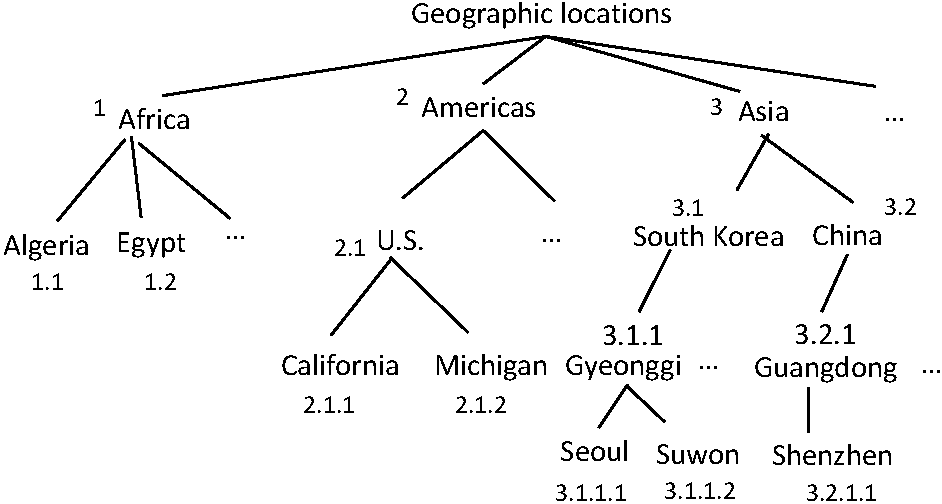
\includegraphics[width=0.45\textwidth]{figures/taxonomylabels}
 \caption{An example of geographical taxonomy with labels}
\label{fig:toytaxonomyexample}
\end{figure}


A string join, which finds all equivalent string pairs between two input collections, is an essential operation in many applications, such as  data integration \cite{conf/sigmod/Sarawagi04}, data cleansing \cite{conf/vldb/ArasuGK06,journals/www/LiJM06} and record linkage \cite{books/Winkler99}. In practice, the same object/entity may have different representations  due to a variety of reasons such as misspellings
caused by typographic errors and different formatting conventions including synonyms, abbreviations and acronyms. Hence, it is important to support approximate string joins for reconciling different
representations of an entity. A large number of  similarity functions such as Levenshtein distance~\cite{conf/sigmod/WangLF12},
Hamming distance~\cite{conf/spire/Kondrak05}, Episode
distance~\cite{conf/ijcai/CohenRF03}, Cosine
metric~\cite{journals/ipm/SaltonB88}, Jaccard
Coefficient~\cite{conf/icde/ChaudhuriGK06,conf/icde/LiLL08}, JaccT \cite{conf/icde/ArasuCK08} and Synonym-based similarity \cite{conf/sigmod/LuLWLW13} have been proposed in the literature. It is well known
that no single similarity function is universally applicable
across all domains and scenarios.

In this paper, we investigate a novel problem to exploit taxonomy with string similarity joins. In principle, the taxonomy presents a general purpose strategy to improve the accuracy of string joins by enriching data with semantics-based knowledge. Taxonomies are sets of IS-A hierarchies, which identify the relations between different concepts. The IS-A relationship
is a transitive closure of the concept-instance relationship.
For example, if ``\textsf{kitten}'' is an instance of ``\textsf{cat}'', and
``\textsf{cat}'' is an instance of ``\textsf{pet}'', then ``\textsf{kitten}'' is an instance
of ``\textsf{pet}''. If we treat each term as a node, and create
for each (concept, instance) pair, an edge from the concept
to the instance, then we can think of the taxonomy as a tree or forest. For any node that representing a term,
the IS-A relation could be any descendant of it in the tree. Figure
\ref{fig:toytaxonomyexample} gives a toy example of a geographical taxonomy tree.

Based on the taxonomy,  the similarity of two strings can be measured in a \textit{semantic} way. For example, consider two pairs (\textsf{Los Angles}, \textsf{Cupertino}) and (\textsf{Los Angles}, \textsf{Seoul}). Intuitively, the similarity between \textsf{Los Angles} and \textsf{Cupertino} should be greater than that between \textsf{Los Angles} and \textsf{Seoul}, because the formers are two cities in the same country and the same state. To quantify the similarity, one method is to calculate the longest common prefixes (LCP) between two strings against the taxonomy. Thus, based on Figure \ref{fig:toytaxonomyexample}, LCP(\textsf{Los Angles}, \textsf{Cupertino})= 4, but (\textsf{Los Angles}, \textsf{Seoul})=1. Clearly the similarity between \textsf{Los Angles} and \textsf{Cupertino} is greater than that between \textsf{Los Angles} and \textsf{Seoul}.


\begin{figure}[t]
\centering
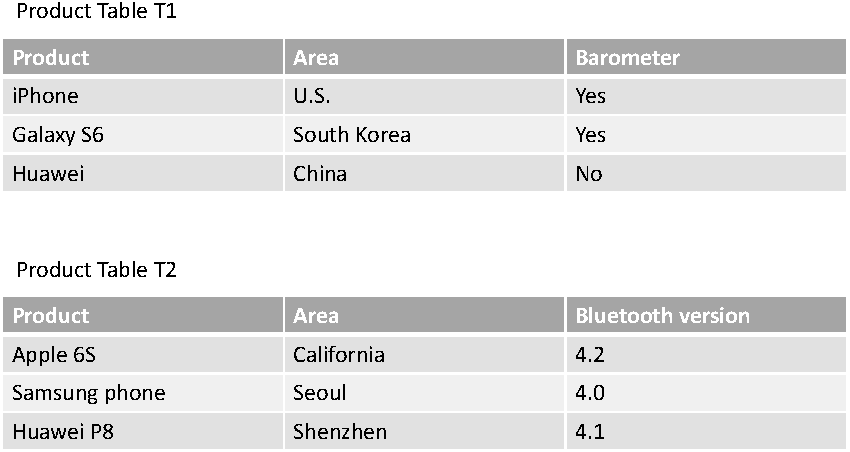
\includegraphics[width=0.45\textwidth]{figures/productexample}
 \caption{Two tables for data integration}
\label{fig:twotables}
\end{figure}

We give several applications to shed light on the importance of the  string similarity matching with taxonomy on databases.

\begin{itemize}
  \item \textbf{Data Integration} ~ Data integration involves combining data residing in different sources. Taxonomy is quite useful to  discover the relations of various objects. For example, consider two tables in Figure \ref{fig:twotables}. In order to correctly perform the integration between two tables, the system needs to know hat ``\textsf{Apple 6s is a model of iphone}'' and ``\textsf{Cupertino is a city in US}'', and etc. A join mechanism that can utilize such taxonomy knowledge may help users to discover more relevant records and thus to improve the effectiveness of data integration.
  \item \textbf{Data mining} ~ Term classification and term clustering are two important tasks in data mining. A new similarity measure that can find the IS-A relations between terms is beneficial to term classification and clustering algorithms to improve their accuracies \cite{journals/dke/CaglieroG13}.
  \item \textbf{Data cleaning}~  Data cleaning is the process of detecting and correcting (or removing) corrupt or inaccurate records from a table or database. Two records about ``\textsf{Sumsung cellphone}'' and ``\textsf{Glaxy S6}'' may contain the duplicate or inconsistent information, because ``\textsf{Glaxy S6}'' IS-A model of ``\textsf{Sumsung cellphones}''. In those scenarios, the taxonomy enhances the quality of data cleaning by finding more relevant records.

\end{itemize}

  %\item \textbf{Information extraction} Find all geological entity in U.S. Then a new similarity measure based on a geological taxonomy can handle term variation and discover more location of interests


%  Conceptually, there are two cases of string joins: \textit{exact-joins} and \textit{approximate-joins}. Exact joins mean that two matching strings are exactly the same, while approximate joins tolerate certain difference between two strings and the similarity between two strings is measured by a similarity function, such as  Levenshtein distance~\cite{conf/sigmod/WangLF12},
%Hamming distance~\cite{conf/spire/Kondrak05}, Episode
%distance~\cite{conf/ijcai/CohenRF03}, Cosine
%metric~\cite{journals/ipm/SaltonB88}, Jaccard
%Coefficient~\cite{conf/icde/ChaudhuriGK06,conf/icde/LiLL08}, and Dice
%similarity~\cite{conf/www/BayardoMS07}.



In this paper, we assume that we already have complete
information of these IS-A relations, i.e. \textit{taxonomy}, and we will focus on how
to efficiently perform a string join by utilizing the taxonomy, and how to optimize the index structure
for this purpose.

%For example, the (Guangdong, Shenzhen) is a (concept, instance) pair and (Shenzhen, China) has the IS-A relation, as Shenzhen is a city in China.


To support the string joins with taxonomy, the first step is to devise new similarity functions which can utilize the taxonomy. Although there is a wealth of research on string similarity functions, most of them focus only on the syntactical-level of words. Some emerging works  \cite{conf/icde/ArasuCK08} can utilize the synonyms to performs the string join, which use semantic information for word comparing. But their works cannot be easily extended to handle taxonomy, because  taxonomy represent a tree-like structure, which is more complicated than the binary relations as specified in synonyms (See Section 2 for more explanations of why the existing similarity functions are not applicable for taxonomy).



%\noindent which selects the prices of phones from two tables by performing the two IS-A joins against ``\textsf{product}'' and %``\textsf{area}'' columns (e.g. ``\textsf{Galaxy S6}'' is a model of ``\textsf{Samsung}'' in the \texttt{product} column and %``\textsf{Seoul}'' is a city of ``\textsf{South Korea}'' in the \texttt{area} column).

We first define the similarity between two nodes in the taxonomy, then we use the maximum weighted bipartite model to define the similarity of two strings.

Given the newly similarity functions TS and ETS, it is imperative to study efficient similarity join algorithms. The brute-force algorithm that enumerates every string pair and checks whether the two strings in the pair are similar is rather expensive. To alleviate this problem, many algorithms have been proposed in the recent two decades. One widely-adopted technique employs a filter-verification framework, which includes two steps: (1) Filter step: devising effective filtering algorithms to prune large numbers of dissimilar pairs and generating a set of candidate pairs; and (2) Verification step: verifying each candidate pair by computing
the real similarity and outputting the final results. Filtering algorithms in the first step play an important role
in the framework. Most of existing filtering algorithms employ a signature-based technique, which generates signatures for each string such that if two strings are similar, their signatures must have overlaps. Thus the signature-based technique can prune string pairs that have no common signature.

Recently many filtering techniques have been proposed, e.g., count filtering [8,13,18], length filtering [8,14], position
filtering [25,27], prefix filtering [4] and content filtering [25]. As prefix filtering is the most effective filtering technique,
many algorithms have been proposed to optimize prefix filtering for different similarity metrics, e.g., AllPair [2],
PPJoin [27], EDJoin [25], QChunk [17], VChunk [24], AdaptJoin [23]. There are also many other signature schemes, e.g., PartEnum [1],
PassJoin [14], FastSS [20].

Unfortunately, these algorithms are not easily extended to process taxonomy. Because all the existing methods are based on the observation that two strings are similar only if their signatures overlap. But this is not true for taxonomy, because two strings may have IS-A relation without any common tokens (signatures).

Our technical contribution here is to propose a new filtering strategy based on ETS similarity function. We first extend prefix scheme to propose n-ary prefix scheme. This n-ary prefix scheme has the independent interests in that it can outperform the state-of-art algorithms  for similarity joins even without the taxonomy. And then introduce the taxonomy node into the signature set and generate a composite signature scheme. We show that our n-ary prefix
filter has larger pruning power and less filtering cost
than state-of-the-art filters in a theoretical analysis based on Jaccard similarity.


Finally, we perform experiments to evaluate our results and show the benefits of proposal algorithms.

%\subsection{Novelty and contributions}
%
%Our contributions are as follows.
%\noindent \textbf{Introduction of taxonomy for string joins}. We introduce a new problem to utilize the taxonomy for the string joins in databases, which has application in data integration and data cleansing. We propose a novel
%
%\noindent \textbf{Optimal algorithms for TS} We develop an inverted list introduce an algorithm for multiple string joins.
%
%\noindent \textbf{Novel filters for ETS function} We extend TS to handle more general cases of strings with taxonomy and propose a composite n-ary signatures.
%
%\noindent \textbf{Generality and variations}  We introduce a novel algorithm for incrementally updating taxonomy. Our merging algorithm allows us to incorporate new correlations introduced over a subset of tuples into
%the correlations already present in the database, without recomputing the existing results.



\smallskip

The rest of this paper is organized as follows. Section 2
provides the necessary definitions, formulates . Section
3 includes our algorithm for exact joins with taxonomy. In Section 4, we study
the approximate string join, proposing our solution, analyzing its approximation
ratio, and presenting our similarity join algorithms.
Our experiments are presented in Section 5. Finally,
Section 6 concludes with a discussion about future work.


\section{Related work} \label{sec:relatedwork}

Taxonomy is the practice and science of classification. Many taxonomies have a hierarchical structure, but this is not a requirement. In this work, we study to leverage the existing taxonomy to improve the accuracy of string record join in databases. Such a taxonomy could be constructed manually
through experts and community efforts, as in WordNet
[4], Cyc [14], and Freebase. With the advantage of freshness
and informativeness, automatic taxonomy construction has
been extensively studied recently, for example, in [20, 22,
18, 21, 26]. WikiTaxonomy [18] and YAGO [22] may be the
most notable efforts, which attempt to derive a taxonomy
from Wikipedia categories. With more web data, Probase
[26] aims at building a unified taxonomy of worldly facts.

In recent years, we have witnessed the emergence of various efforts to enhance the effectiveness of string similarity joins by using synonyms \cite{conf/sigmod/LuLWLW13,conf/icde/ArasuCK08,conf/cpm/BarbayGMR06,conf/vldb/ArvindSR09}.
The traditional similarity functions consider only syntactic similarities, e.g., number of common
words or $q$-grams. But there are many important cases where syntactically different
strings can represent the same real-world object. For example,
``\textsf{Bill}'' is a short form of ``\textsf{William}'', and ``\textsf{ICDE}'' is an abbreviation of  ``\textsf{International Conference on Data Engineering}''.  Given two collections of strings,  synonym-based similarity functions can utilize the available synonyms to find string pairs which are semantically similar. While those methods improve the effectiveness of string joins, a synonym dictionary does not contain information such as
``\textsf{Helsinki is the capital of Finland}'', or `\textsf{`Apple 6 Plus is a new model of iPhone}''. Still, term pairs such as ``\textsf{Helsinki}'' and ``\textsf{Finland}'', ``\textsf{Apple 6 Plus}'' and ``\textsf{iPhone}''  have strong semantic correlations.



Taxonomies are is-a hierarchies of concepts, topics, or keywords. Since they represent ontology specializations, they may be
used to provide meaningful knowledge representations and, thus, support users in understanding the semantic meaning of a
resource and the related domain.
Several efforts to integrate taxonomies in the Data mining and Knowledge Discovery (KDD) process have been done. For
instance, taxonomies have already been exploited to (i) discover high level correlations among data [9�C13], (ii) perform textual
data analysis and summarization [14,15,35,36], (iii) improve user browsing by looking into the results of Web search engines
[37], and (iv) enhance the quality of recommendation systems [17,38]. This paper focuses on exploiting taxonomy information to
enrich data used for classification. To the best of our knowledge, it is the first attempt to integrate high level and multi-faceted
knowledge into classifier construction.


Several types of Similarity Join have been proposed in the
literature, e.g., distance range join (retrieves all pairs whose distances
are smaller than a predefined threshold $\varepsilon$) [2, 3, 4, 5, 6,
7], k-Distance join (retrieves the k most-similar pairs) [8], and
kNN-join (retrieves, for each tuple in one table, the k nearest neighbors
in another table) [9, 10, 11]. The distance range join
has been one of the most studied and useful types of Similarity
Join. This type of join is commonly referred to simply as Similarity
Join and is the focus of this paper. Among its most relevant
implementation techniques, we find approaches that rely
on the use of pre-built indices, e.g., eD-index [3], D-index [4],
and List of Twin Clusters (LTC) [12]. These techniques strive
to partition the data while clustering together the similar objects.
While these indexing techniques support the SJ operation
they also have some shortcomings: D-index and eD-index may
require rebuilding the index to support queries with different $\varepsilon$,

Approximate string matching includes finding (sub)strings
that resemble a given query string. It is a well-researched
topic and has many applications, such as data cleansing [1],
spelling correction [19], query autocompletion [33], near duplicate
detection [25, 32], approximate named entity recognition
[29], and bioinformatics [20, 27, 35].
Due to the sheer amount of literature in this area, we will
focus on most related recent results and refer readers to the
excellent surveys [13, 22] and tutorials [3, 12, 16] for a comprehensive
treatment of the topic.
Based on the types of the queries, recent work focuses either
on efficient single query processing (typically named string
similarity queries) [1, 6, 9, 11, 18, 25, 28, 31], or the similarity
join which can be treated as processing a batch of similarity
queries [2, 8, 10, 12, 14, 17, 28, 29, 34, 35]. Most recently,
Jiang et al. [15] experimentally evaluate and analyze many of
the existing similarity join algorithms.


$\mathbf{Prefix filter.}$ Since the prefix
filter is effective, many methods are proposed to optimize it
for different similarity operators. ED-
join [12,28] proposed a location-based mismatch filter to re-
duce prefix length and a content-based mismatch filter to
reduce the number of candidates for ED. Pivotal prefix filter [4] reduced the prex length for ED. PassJoin [17] pro-
posed segment filter to improve pruning power. PPJoin [29]
used the positions of prefix and suffix to improve pruning
power for token-based similarities. Length filter was pro-
posed to prune dissimilar answers based on length difference [8]. TrieJoin [23] used a different framework that directly computed real similarity using the trie structure.





\section{Preliminaries} \label{sec:preliminaries}



In this section, we first  define taxonomy, including
hypernym and hyponym. Subsequently,
we discuss challenges of processing taxonomy-based approximate string joins.


\subsection{Taxonomy}

A taxonomy (T ,$\sqsubset$ ) consists of a universe of terms T and
a term-term hypernym-hyponym relationship $\sqsubset$.

Hypernym-hyponym relationship. The hypernym-hyponym relationship
$\sqsubset$ is a partial order T . For two terms t1 and t2,
we write t1 $\sqsubset$ t2 or t2 $\sqsubset$ t1, if t1 is a hypernym of t2 (or t2
is a hyponym of t1). For example, ``Caribbean Region'' is a hyponym of
``Americas''. Figure  \ref{fig:taxonomy} shows an example of taxonomy for geological locations.



Hyponymy shows the relationship between the more general terms (hypernyms) and the more specific instances of it (hyponyms). A hyponym is a word or phrase whose semantic field is more specific than its hypernym. The semantic field of a hypernym, also known as a superordinate, is broader than that of a hyponym. An approach to the relationship between hyponyms and hypernyms is to view a hypernym as consisting of hyponyms. This, however, becomes more difficult with abstract words such as imagine, understand and knowledge. While hyponyms are typically used to refer to nouns, it can also be used on other parts of speech. Like nouns, hyponyms in verbs are words that refer to a broad category of actions. For example, verbs such as stare, gaze, view and peer can also be considered hyponyms of the verb look.
Hypernyms and hyponyms are asymmetric. Hyponymy can be tested by substituting X and Y in the sentence ``X is a kind of Y'' and determining if it makes sense.[4] For example, ``A screwdriver is a kind of tool''  makes sense but not ``A tool is a kind of screwdriver''.


Hyponymy is a transitive relation, if X is a hyponym of Y, and Y is a hyponym of Z, then X is a hyponym of Z.[5] For example, violet is a hyponym of purple and purple is a hyponym of color; therefore violet is a hyponym of color. In addition, it should be noted that a word can be both a hypernym and a hyponym: for example purple is a hyponym of colour but itself is a hypernym of the broad spectrum of shades of purple between the range of crimson and violet.

The hierarchical structure of semantic fields can be mostly seen in hyponymy. They could be observed from top to bottom, where the higher level is more general and the lower level is more specific. For example, living things will be the highest level followed by plants and animals, and the lowest level may comprise dog, cat and wolf.

Under the relations of hyponymy and incompatibility, taxonomic hierarchical structures too can be formed. It consists of two relations; the first one being exemplified in 'An X is a Y' (simple hyponymy) while the second relation is 'An X is a kind/type of Y'. The second relation is said to be more discriminating and can be classified more specifically under the concept of taxonomy.

Computer science often terms this relationship an ``is-a'' relationship. For example, the phrase ``Red is-a colour'' can be used to describe the hyponymic relationship between red and colour.

Hyponymy is the most frequently encoded relation among synsets used in lexical databases such as WordNet. These semantic relations can also be used to compare semantic similarity by judging the distance between two synsets and to analyse Anaphora.

As a hypernym can be understood as a more general word than its hyponym, the relation is used in semantic compression by generalization to reduce a level of specialization.

%\begin{figure}[t]
%\centering
%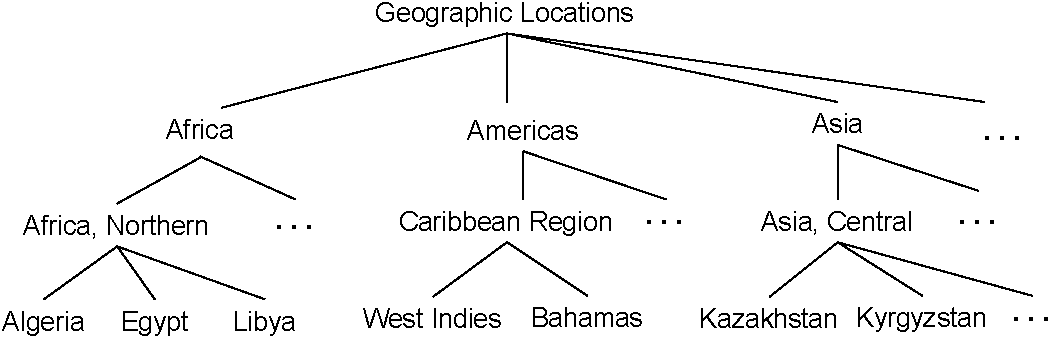
\includegraphics[width=0.45\textwidth]{figures/taxonomy}
% \caption{An example of taxonomy on ``\textsf{Geographic locations}''}
%\label{fig:taxonomy}
%\end{figure}
%
%Example extended SQL
%
%Select  T1.price, T2.price \\
%From Table T1 and T2 \\
%Where T1.area is\_a\_hypernym T2.area \\
%With taxonomy T \\
%
%
%The second SQL query:
%
%Select  T1.price, T2.price, T3.price \\
%From Table T1, T2, T3 \\
%Where T1.area is\_a\_hypernym T2.area AND T1.product is\_a\_hypernym T2.product
%



\section{String joins with taxonomy}

We consider the exact joins including hypernymy and hyponymy and mixed three predicates based on taxonomy T.



The baseline join algorithm is the nested-loop join. All string pairs are accessed to determine the hyper-hypo relationships. But this algorithm is obviously not efficient. Therefore, we propose an efficient algorithm.



\begin{figure}[t]
\centering
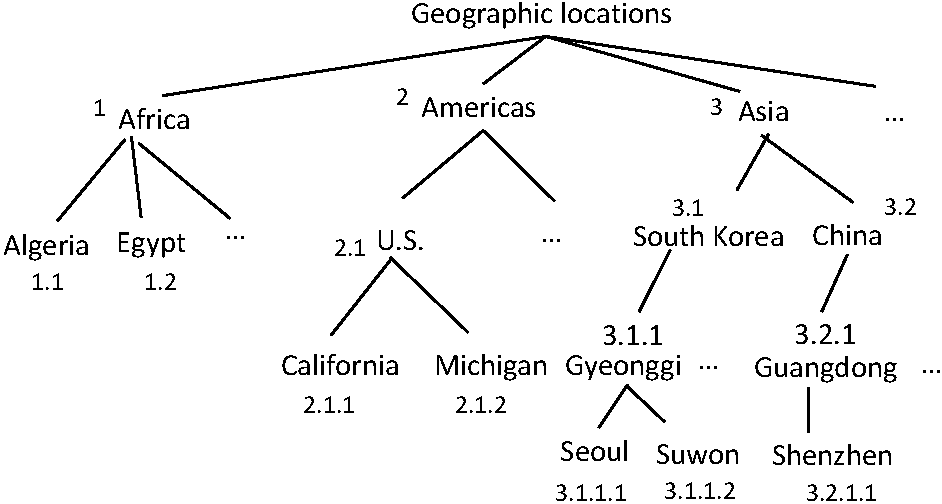
\includegraphics[width=0.45\textwidth]{figures/taxonomylabels}
 \caption{An example of taxonomy with labels}
\label{fig:taxonomy}
\end{figure}



\begin{figure}[t]
\centering
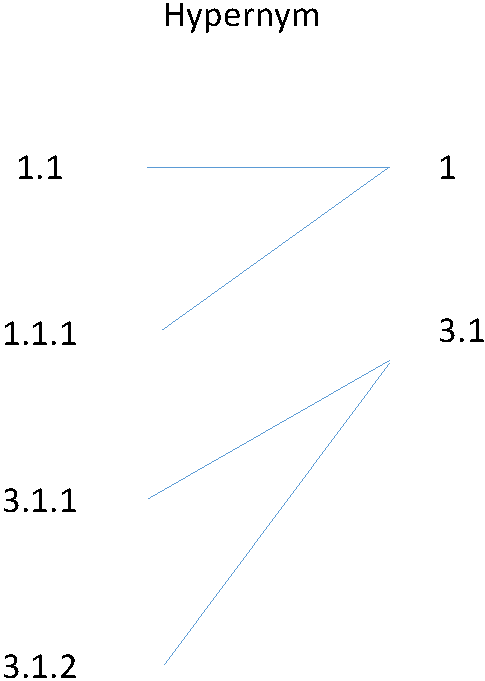
\includegraphics[scale=0.4]{figures/labeljoins}
 \caption{Join inverted lists}
\label{fig:taxonomy}
\end{figure}


%\begin{algorithm}
%{\bf Input}: two strings $s_1$ and $s_2$ \\
%{\bf Output}: four relationships: R=\{Hype, Hypo, Equa and Non\}
%\begin{compactenum}[(1)]
%\item {\bf If} ($s_1 = s_2$ )  {\bf return} Equa;
%\item {\bf If} ($|LCD(s_1)| >$ 1 AND $|LCD(s_2)| >$ 1 )  {\bf return} None;
%\item {\bf Else} {\bf if} ($|LCD(s_1)| =$ 1 AND $|LCD(s_2)| >$ 1 )
%\item \verb"  " {\bf If}  $\forall t \in LCD(s_1)$, $t$ is a hypernym of $LCD(s_2)$
%\item \verb"    " {\bf return} Hype {\bf else} {\bf return} None;
%\item {\bf Else} {\bf if} ($|LCD(s_2)| =$ 1 AND $|LCD(s_1)| >$ 1 )
%\item \verb"  " {\bf If}  $\forall t \in LCD(s_2)$, $t$ is a hypernym of $LCD(s_1)$
%\item  \verb"    " {\bf return} Hypo {\bf else} {\bf return} None;
%\item {\bf Else} /\ *  $|LCD(s_1)| = |LCD(s_2)| = $ 1 */\
%\item  \verb"  " {\bf If}  $LCD(s_1)$ is a hypernym of $LCD(s_2)$  {\bf return} Hype
%\item   \verb"  " {\bf Else if}  $LCD(s_1)$ is a hyponym of $LCD(s_2)$  {\bf return} Hypo
%\item   \verb"  " {\bf Else return} none
%\end{compactenum}
%\caption{Determine the relationship between two strings}
%\label{alg:measure}
%\end{algorithm}


\begin{algorithm}
{\bf Input}: two sets of strings $S_1$ and $S_2$, a taxonomy $T$ \\
{\bf Output}: string pairs $(s_1,s_2) \in S_1 \times S_2$ s.t. $s_1 \sqsubset s_2$ or $s_2 \sqsubset s_1$
\begin{compactenum}[(1)]
\item Let $G_s$ and $G_t$ denote the inverted lists for S and T respectively.
\item Perform a join operation to find the IS-A relationship between $G_s$ and $G_t$
\item {\bf FOR} EACH join pair ($t_1,t_2$)
\item  $R = R \cup t_1.List \times t_2.List$
\item $R$
\end{compactenum}
\caption{String joins with taxonomy}
\label{alg:exactjoin}
\end{algorithm}

Note that the above algorithm may contain the duplicate result set. Therefore, we need to sort and remove the duplication.

\begin{theorem}  Algorithm \ref{alg:exactjoin} is an optimal algorithm. The computing cost is linear to the sum of the size of the input and output. That is, each output result contribute to the final answer.
\end{theorem}

\subsection{Join algorithms}

The key to an efficient, uniform mechanism for set-at-atime
(join-based) matching of query graph patterns is a positional
representation of occurrences of  elements and in the taxonomy database (see, e.g., [6, 7, 27]),
which extends the classic inverted index data structure in information retrieval [22]. We borrow the labeling scheme from XML databases and use the prefix based labels. Structural relationships between tree nodes whose positions
are recorded in this fashion can be determined easily for hypernym or hyponym relationships.

There are two kinds of edges in a graph pattern, ``$\rightarrow$'' and ``$\leftarrow$''shows the IS-A relationship, hypernym and hyponym and ``$\leftrightarrows$'' is a mixedISA relationship.

In general, at each node in the query graph pattern, there is
a node predicate on the attributes (e.g., tag, content) of the
node in question. For the purposes of this paper, exactly
what is permitted in this predicate is not material.  It suffices
for our purposes that there be efficient access mechanisms
(such as index structures) to identify the nodes in the
database that satisfy any given node predicate $q$, and
return a stream of matches $T_q$ based on the taxonomy.


\section{String similarity joins with taxonomy}


In this section, we discuss how to use taxonomy on string similarity joins. For this purpose, we first extend the Jaccard similarity to utilize the taxonomy. Then we propose several algorithms and optimizations for the problem of similarity joins with taxonomy.



\subsection{Similarity measures}


We define the taxonomy similarity between two strings:

\begin{definition}[Taxonomy intersection]
Given two token sets $S_1$ and $S_2$, and a taxonomy $\mathcal{T}$, we say an element (token) $e \in S_1 \bigcap_T S_2$, if $ \exists E \subseteq S_1$ and $e \in E$, and $\exists T \subseteq S_2$, s.t. $\exists (E,T) \in \mathcal{T}$.\end{definition}


\noindent \textbf{Remark.}  Given two strings $s$ and $t$, it is clear that $|s \cap t| \leq min (|s|,|t|)$. But based on the taxonomy intersection, it is possible that $|s \cap_T t| > |s| $ or $|s \cap t| > |t| $. For example, s=``California'', t=``U.S.'', $|s \cap_T t|$ = 2. But it is still true that $|s \cap_T t| < |s \cup t|$

We need to define a new similarity:

Given a token set S which include two parts: $S_1$ and $S_2$, where $S_1$ contains only unique token and $S_2$ is the taxonomy token. Then the similarity between S and T is defined as

$\frac{min(|S_2|,|T_s|)}{|S_1|+|T_1|+min(|S_2|,|T_s|)}$

\begin{definition}[Taxonomy-based Jaccard]   Given two sets of tokens $S_1$ and $S_2$,  the taxonomy-based Jaccard (TJ) between $S_1$ and $S_2$ is that:

\begin{equation}
TJ(S_1,S_2)=  \frac{(S_1 \bigcap_T S_2) \bigcup (S_1 \bigcap S_2) }{S_1 \bigcup S_2}
\end{equation} \end{definition}

\begin{algorithm}
{\bf Input}: two strings $s_1$ and $s_2$, a taxonomy $\mathcal{T}$ \\
{\bf Output}: $TJ(s_1,s_2,\mathcal{T})$
\begin{compactenum}[(1)]
\item Let $S_T $ to contain all tokens for taxonomy-based intersection. Initially, $S_T = \emptyset$.
\item Let $L_1$ (resp. $L_2$) denote the applicable taxonomy node list for $s_1$ (resp. $s_2$);
\item Scan $L_1$ and $L_2$ sequentially to find any matching pair $n_1 \in L_1$, $n_2 \in L_2$, s.t. ($n_1$,$n_2$) has the IS-A relation in $\mathcal{T}$;
\item Add all tokens $t \in n_1 \cup n_2$ to the set $S_T$;
\item  return $\frac{S_T \cup (|s_1 \cap s_2|)}{|s_1 \cup s_2|}$;
\end{compactenum}
\caption{String joins with taxonomy}
\label{alg:exactjoin}
\end{algorithm}

The time complexity of the TJ is $O(|s_1|+|s_2|+|n_1|+|n_2|)$, where $n_1$ (resp. $n_2$) denotes all applicable taxonomy nodes for string $s_1$  (resp. $n_2$). Assume that the preprocessing step finds the taxonomy relation for each string. Then the online algorithm only needs to find the matching IS-A relation between two strings to compute the intersection set with taxonomy.

\subsection{String similarity join algorithms}


%\begin{figure}[t]
%\centering
%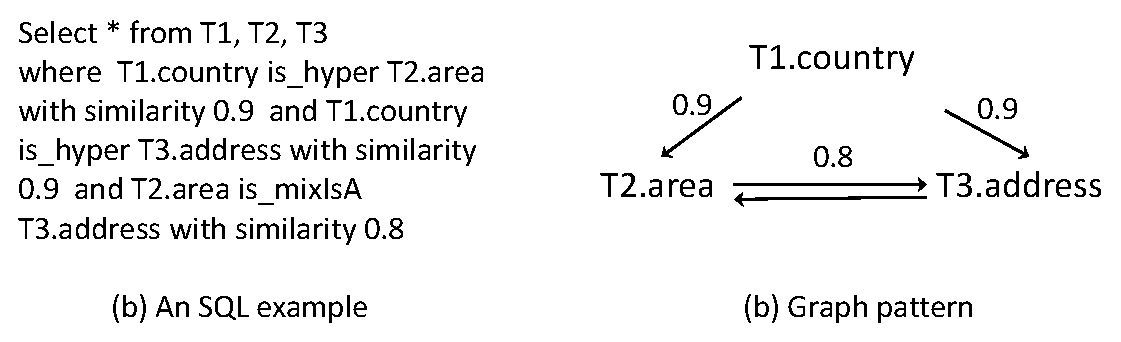
\includegraphics[scale=0.4]{figures/tgsql2}
% \caption{Taxonomy graph example }
%\label{fig:similaritygeaph}
%\end{figure}

We would formulate the string similarity join problem and develop the corresponding algorithms. Given two collections of strings $S$ and $T$, a taxonomy tree
$\mathcal{T}$, and a similarity threshold $\theta$, a \textit{string
  similarity join} finds all string pairs $(s, t) \in S \times T$,
such that $JT(s,t,\mathcal{T})$ $>$ $\theta$, where \textit{JT} is
 the Jaccard-taxonomy similarity functions defined above. Two join algorithms would be proposed in the following subsections.



\textbf{Baseline algorithm}. We can use the similar algorithm as that in string exact join with taxonomy. And then use these candidate for filtering. But this baseline algorithm has one limitation that there are too many candidates. Then we show how to perform the second filtering to reduce the number of candidate pairs.

\textbf{Signature-based index}. Given a string s with length $|s|$, then the size of signature is $\lceil (1-\theta)|s| \rceil$. But if the signatures involve the taxonomy, then we cannot make this argument.

But if in some real cases, we select the word from taxonomy as signatures. Therefore we need to compute a relax maximum similarity. In this case, we still do not need to retrieve the whole string to compute real similarity.

Given as string $s$, assume that its applied taxonomy node is $n$.

In this paper, we propose a new index which combine a signature filters and a length together with a bit-matrix, which extends bloom filter to two dimensions.

In the literature, the current "modus operandi" is called \textit{prefix filter}, which is based on the intuition that if two canonicalized records are similar, some fragments of them should overlap with each other, as otherwise the two records
won't have enough overlap. This intuition can be formally captured by the prefix-filtering
principle \cite{conf/icde/ChaudhuriGK06} rephrased below.

\begin{lem} (\textsc{Prefix filter principle}) \cite{conf/icde/ChaudhuriGK06} Given an
ordering $O$ of the token universe $U$ and two strings $s$ and $t$, each with tokens sorted in the
order of $O$.   If Jaccard($s, t$) $> \theta$, then the first $\lceil(1-\theta)|s|\rceil$ smallest
tokens of $s$ and the first $\lceil(1-\theta)|t|\rceil$ smallest
tokens of $t$  must share at least one token.
\end{lem}

\subsubsection{N-ary prefix scheme}




Given a string $s$, we can construct the $n$-ary prefix token combination as follows:  Given an
ordering $O$ of the token universe $U$, we select $n$ tokens from the first $\lceil (1-
\theta) \cdot |s| \rceil + n -1$ in $s$. Then let $B^s_n$ denote the set to contain all $n$-combinations. That is  $|B^s_n|$= $\binom{(1-\theta)|s|+n-1}{n}$.

\begin{lem} (\textsc{N-ary signature principle}) Given two strings $s$ and $t$ and their n-ary signatures $T^s$ and $T^t$ respectively, if Jaccard($s, t$) $> \theta$, then $T^s \cap T^t \neq \emptyset$.
\end{lem}

Given a string s=\{A,B,C,D,E\}. If we use the prefix filtering, then the signature is A and B. Assume that $\theta$=0.75, (1-0.75)*5=1.25 and $\lceil 1.25 \rceil$=2. But in our bi-tuple scheme, we select two tokens as the signatures, including \{A,B\},\{A,C\},\{B,C\}.

Similarly, we can develop a 3-tuple signature. we select three tokens as the signatures, including $\binom{4}{3}$=4, i.e. \{A,B,C\}, \{A,C,D\}, \{B,C,D\}, \{A,B,D\}.

Furthermore, we can extend to 4-tuple signature, that is $\binom{5}{4}$=4, i.e. \{A,B,C,D\}, \{A,C,D,E\}, \{A,B,D,E\}, \{A,C,D,E\}, \{B,C,D,E\}.

One question is how to select the number $n$ for n-tuple scheme. What is the optimal value of $n$? Let $t= (1-\theta)|s|$, that is, $O((t+n-1)^{n})$. If n is too large, then there are many signatures, it may not be an optimal solution. Therefore, the key point is how to decide a good $n$?


\subsubsection{N-ary prefix scheme with taxonomy}

 Given a string s=\{A,B,C,D,E\}, assume that we use 3-tuple signature, $\binom{4}{3}$=4, i.e. \{A,B,C\}, \{A,C,D\}, \{B,C,D\}, \{A,B,D\}.

For each tokens, there are two cases, that is, it contains a taxonomy word, say $t \in w$. Then we use $w$ to replace $t$. Note that $t$ may belong to multiple taxonomy words. Therefore, ($w_1, w_2, \cdots, w_3$)

Continue the above example, assume that $DE$ = 1.1. Note that $E \in s $, but $E$ does not belong to the signatures. Then the new three signatures:  \{A,C,1.1\}, \{B,C,1.1\}, \{A,B,1.1\}.

\noindent \textbf{Composite signatures} Given a string $s$, a composite signature of $s$, denoted by C-Sig($s$) includes two types of elements $T$ and $N$, where $T$ is a set of tokens and $N$ is a set of T-nodes.

Given an
ordering $O = (U_1 , U_2 )$ of the token universe $U_1$ and $U_2$, where $U_1$ denotes the set of non-taxonomy tokens and $U_2$ is the set of taxonomy tokens. Let $P_s$ denote the smallest $\lceil(1-\theta)|s|\rceil$ tokens.

%\begin{lem} (\textsc{Prefix filter principle with taxonomy})  Given two strings $s$ and $t$ with n-ary prefix signatures, if TJ($s, t$) $\geq \theta$, then one of the following cases holds:
%
% \begin{itemize}
%   \item $P_s \cap P_t \neq \emptyset$, or
%   \item  $T_s \cap A_t \neq \emptyset$ or $T_t \cap A_s \neq \emptyset$
% \end{itemize}
%
%\end{lem}
%


%\begin{lem} (\textsc{Prefix filter principle with taxonomy})  Given two strings $s$ and $t$ with n-ary prefix signatures, if TJ($s, t$) $\geq \theta$, then one of the following cases holds:
%
% \begin{itemize}
%   \item $P_s \cap P_t \neq \emptyset$, or both of the conditions satisfy:
%   \item  $\exists sig^s \in P_s, sig = sig^s_{token} \cup sig^s_{tax} s.t. \exists sig^t \supseteq sig^s$ and $sig^s_{tax} \subseteq Tax(t)$ and
%    \item  $\exists sig^t \in P_t, sig = sig^t_{token} \cup sig^t_{tax} s.t. \exists sig^s \supseteq sig^t$ and $sig^t_{tax} \subseteq Tax(s)$
% \end{itemize}
%
%\end{lem}

A signature set $P$ for a string $s$ is a binary tuple ($T,N$), where $T$ is a set of tokens and $N$ is a set of taxonomy nodes.

\begin{definition} [Signatures match strings]
Given a signature set $P = (T,N)$ and a string $s$, we say $P$ matches $s$, denoted by $P \vdash s$ if $N \subseteq N^s$, where $N^s$ is a set of applicable taxonomy nodes of $s$ and  there exits a signature set $P' = (T',N')$ of $s$, s.t. $T \subseteq T'$.
\end{definition}


\begin{lem} (\textsc{Composite signatures principle})  Given two strings $s$ and $t$ with signatures $P^s$ and $P^t$ respectively, if TJ($s, t$) $> \theta$, then $P^s \vdash t$ and $P^t \vdash s$.

\end{lem}

For example, consider two strings s=\{A,B,C,D,E\} and t=\{F,G\}. Assume that $t_1$ = (ACD,G) is an IS-A relation and the $|s \cap_T t| $=4, $JT(s,t)$ = $\frac{4}{7}$= 0.57.
If the threshold $\theta =$ 0.5, then  $\lceil (1-\theta) \times 5 \rceil$= 3 for $s$ and $\lceil (1-\theta) \times 2 \rceil$= 1. Assume that the order of non-taxonomy tokens $O_1$= \{$B, E, F$\} and the order of taxonomy tokens is $O_2$ = \{$A, C, D, G$\}. So the signature of $s$ is \{B,E,A\}, and an IS-A relation $T_s$ = (ACD,G). The signature of $t$ is \{F\} and $A_t$ = (ACD,G). $ T_s \cap A_t \neq \emptyset$.

\subsubsection{Similarity join algorithm}

We discuss the similarity join algorithm based on the above n-ary composite signature filters.


\begin{algorithm}
{\bf Input}:  two collections of strings $S$ and $T$ and the threshold $\theta$ \\
{\bf Output}: result pairs ($s,t$)$\in S \times T$, s.t. JT($s,t$)$> \theta$
\begin{compactenum}[(1)]
\item Find candidate pairs $C_1$ = \{$(s,t) |$  $P^s \vdash t$\};
\item Find candidate pairs $C_2$ = \{$(s,t) |$  $P^t \vdash s$\};
\item  $C= C_1 \cap C_2$;
\item FOR EACH ($s,t$)$\in C$
\item RETURN all pairs s.t. $JT(s,t) > \theta$
\end{compactenum}
\caption{String joins with taxonomy}
\label{alg:exactjoin}
\end{algorithm}

For each table, we can generate four inverted lists for strings: (1) a list $L_I$ for tokens where the signatures of strings contain only tokens; (2) a list $L_{II}$ for taxonomy nodes where the signatures of strings contain only nodes; (3) a list $L_{III}$ for tokens where the signatures of strings contain both tokens and nodes; (4)  a list $L_{IV}$ for nodes where the signatures of strings contain both tokens and nodes.


\begin{algorithm}
{\bf Input}: two collection of strings $S$ and $T$ and their corresponding inverted lists $L_I^S$,  $L_{II}^S$, $L_{III}^S$, $L_{IV}^S$, $L_N^T$ \\
{\bf Output}: string candidate pairs \{$(s,t) |$  $P^s \vdash t$, $s \in S$ and $t \in T$\}
\begin{compactenum}[(1)]
\item  $C_1$=$\displaystyle\bigcup_{g \in L_I^S \cap L_I^t} (L_I^s(g) \times L_I^t(g)) $;
\item  $C_2$=$\displaystyle\bigcup_{n \in L_{II}^S \cap L_N^t} (L_{II}^s(n) \times L_N^t(n)) $;
\item  $C_3$=$\displaystyle\bigcup_{g \in L_{III}^S \cap L_{III}^t} (L_{III}^s(g) \times L_{III}^t(g)) $;
\item  $C_4$=$\displaystyle\bigcup_{n \in L_{IV}^S \cap L_N^t} (L_{IV}^s(n) \times L_N^t(n)) $;
\item   Return $C_1 \cup C_2 \cup (C_3 \cap C_4)$;

\end{compactenum}
\caption{String candidate pairs}
\label{alg:exactjoin}
\end{algorithm}

\begin{table*}[t]
\centering
\begin{tabular}{|@{\hspace{1mm}}c@{\hspace{1mm}}|@{\hspace{1mm}}c@{\hspace{1mm}}|}
%{|p{1cm}|p{1cm}|p{1cm}|p{1cm}|p{1cm}|p{1cm}|p{1cm}|}
%|c|m{6cm}|
\hline
 \textbf{Symbols} & \textbf{Definitions}  \\
  \hline \hline

  $L_I(g)$ &    $\forall s \in L_I(g)$,  s.t. $\exists  R  \in C$-$Sig(s)$, $R$ contains only tokens and $g \in R$ \\

   $L_{II}(n)$ & $\forall$ $s \in L_{II}(n)$, s.t. $\exists  R  \in C$-$Sig(s)$, $R$ contains only T-nodes and $n \in R$    \\

   $L_{III}(g)$ & $\forall$ $s \in L_{III}(g)$, s.t.  $\exists R  \in C$-$Sig(s)$, $R$ contains both tokens and T-nodes, $g \in R$    \\

  $L_{IV}(n)$ &  $\forall s \in L_{IV}(n)$, s.t. $\exists R  \in C$-$Sig(s)$, $R$ contains tokens and T-nodes and $n \in R$    \\

$L_{N}(n)$ &  $\forall s \in L_{N}(n)$, s.t. $n$ is an applicable T-node of $s$   \\

  \hline
\end{tabular}
\caption{Summary of definitions of various inverted lists}
\label{tab:symbols}
\end{table*}


\begin{table*}[t]
\centering
\begin{tabular}{|@{\hspace{1mm}}c@{\hspace{1mm}}|@{\hspace{1mm}}c@{\hspace{1mm}}|@{\hspace{1mm}}c@{\hspace{1mm}}|@{\hspace{1mm}}c@{\hspace{1mm}}|}
%{|p{1cm}|p{1cm}|p{1cm}|p{1cm}|p{1cm}|p{1cm}|p{1cm}|}
%|c|m{6cm}|
\hline
 \textbf{ID} & \textbf{Strings} &  \textbf{Signatures} &    \textbf{C-Sig} \\
  \hline \hline

  $q_1$ & Suwon and Seoul in South Korean  &  (Suwon, and), (Suwon Seoul), (and, Seoul)  & () \\

   $q_2$ & Seoul, South Korean in Asia  & (Seoul, South), (Seoul, Korean), (Seoul, Korean) &   3.1.1.1, in \\

   $q_3$ &  two states: California and Michigan, U.S. &  (two, states), (two, California), (states, California) & (two, states), (two, 2.1.1), (states, 2.1.1)  \\
   $q_4$ & two cities: Detroit and Los angles & (two, cities), (two, Detroit), (cities, Detroit) &  (two, cities), (two, 2.1.2.1), (cities, 2.1.2.1) \\


  \hline
\end{tabular}
\caption{An example to illustrate the string similarity join algorithm}
\label{tab:example}
\end{table*}


\begin{example} We use Table as an example to illustrate the algorithm.

\end{example}

\subsubsection{Comparison with other schemes}


\begin{table}[t]
\centering
\begin{tabular}{|@{\hspace{1mm}}c@{\hspace{1mm}}|@{\hspace{1mm}}c@{\hspace{1mm}}|@{\hspace{1mm}}c@{\hspace{1mm}}|}
%{|p{1cm}|p{1cm}|p{1cm}|p{1cm}|p{1cm}|p{1cm}|p{1cm}|}
%|c|m{6cm}|
\hline
 \textbf{Methods@{}} & \textbf{Signature size} &  \textbf{Filtering power} \\
  \hline \hline

  Prefix & (1 -$\theta$)$|s|$ & Optimal \\


   PartEnum & CPU:  O($1.2002^{|V|} \cdot |V|^{O(1)}$ ) & Optimal \\

   LSH & CPU:  O($|V|$log$|V|$+$|E|$)  & $(2\bar{d}+3)/5$  \\

   Composite Prefix & I/O: O(sort($|E|$+$|V|$))   & No bound \\


  \hline
\end{tabular}
\caption{Time and  I/O cost and performance}
\label{tab:complexity}
\end{table}

 We compare our composite prefix filter with state-of-the-art filters. The objective of the filters is to prune dissimilar strings as many as possible. They require to select a set of q-grams from each of two strings as signatures, denoted as Sig(r) and Sig(s), and compare the two q-gram sets to check whether they share common signatures. Pruning power and filtering cost are two important issues in designing filters.

We first consider the pruning power. One one hand, the smaller the production size of the two signature sets $|Sig(r)| \times$
$|Sig(s)|$, the smaller probability they share common q-grams, and thus the higher pruning power. On the other hand, the number of matching q-grams cannot exceed the smaller signature size of the two strings, min($|Sig(r)|, |Sig(s)|$). Thus
we can use the production size of two signature sets and
the smaller signature set size to evaluate the pruning power. We then evaluate the filtering cost. As the q-gram sets
are sorted, we can use a merge-join algorithm to find the
matching q-grams if there is no index, the filtering cost depends on the sum of signature set sizes of the two strings,
$|Sig(r)|$ + $|Sig(s)|$. Table 3 compares the pruning power and filtering cost of state-of-the-art q-gram-based filters used in AllPair, ED-Join, Qchunk-IndexChunk and Qchunk-IndexGram.

\smallskip

\noindent \textbf{Length filters}


\subsubsection{Composite signature: Performance}

In this section, we cover various aspects of Composite-signature scheme's performance.
We begin by proving that it has good asymptotic performance: For a particular setting of n1 and n2, we can prove
that it provides good filtering effectiveness (i.e., generates only a few false positive candidate pairs) with few signatures per input set.

\begin{theorem} If the Jaccard similarity of two strings are greater than $\theta$, then $Sig(u) \bigcap Sig(v) = \varnothing$ with probability 1-o(1). For this setting of parameters, the number of signature per string is O().
\end{theorem}


Given a $n$-tuple composite filter, we estimate its filtering effectiveness.

We assume that there are $N$ tokens in all tables and the length of each string is $s$.

The possibility of false positive for a string pair $s, t$ is that $P(E_A | E_B)$, $E_B$ means that  $sim(s,t) < \theta$; $E_A$ means that $s$ and $t$ pair cannot be pruned away with the filter.

First consider the 1 prefix signature. We computer $P(E_A, E_B)$, that is, the prefix signature cannot prune away the pair of $Jaccard(s,t) < \theta$

Let $\lambda$ = $(1-\theta)s$ signatures for $t$.

Since $|s| = |t|$ and   $Jaccard(s,t) < \theta$ $\Longleftarrow$ $ |s \cap t| < |s| \cdot \theta$.

%\subsection{Count-Min estimation}
%
%In order to quickly decide if the number of pairs after composite filters, we develop a count-min estimation to quickly determine which $n$ is good for filtering. See the following two examples for joins.
%
%See the example in Figure \ref{fig:signature_example1}. In this example, $\theta$ = 0.8. If we use the 1-element signature, then we cannot prune away any string pair. In signature 2, we use 2-element signature, then there is no candidate. Therefore, the filtering power is better.
%
%Further, when we consider the taxonomy ABCD ISA AGK, shown in Figure \ref{fig:signature_example1}. Then there is one answer pair (s1,t1). The new signature include the taxonomy ID 1.1 and 1  as shown.
%
%\begin{figure}[h]
%\centering
%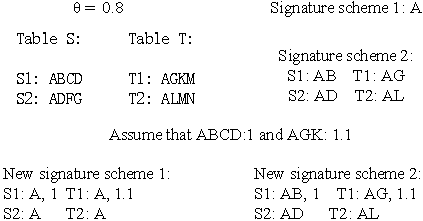
\includegraphics[scale=0.8]{figures/signature_example1}
% \caption{Illustration to the difference of signature schemes}
%\label{fig:signature_example1}
%\end{figure}
%
%A Count-Min (CM) sketch with parameters ( $\varepsilon, \delta$) is represented by a two-dimensional
%array counts with width $w$ and depth $d$. Given parameters ($\varepsilon, \delta$), set
%$w$ = $\lceil \frac{e}{\varepsilon} \rceil$ and $d$ = $\lceil ln \frac{1}{\delta} \rceil $. Each entry of the array is initially zero.
%
%
%When a data item ($w,i$) arrives, meaning that the signature $w$ has the length $i$, then $i$ is added to one cell in each row; the counter is determined by $h_j$. Formally, set $\forall 1 \leq j \leq d$, then count[j,$h_j(i)$]
%
%
%The space used by Count-Min sketches is the array of $wd$ counts, which takes $wd$ words, and $d$ hash
%functions, each of which can be stored using 2 words when using the pairwise functions described in [27].
%
%Estimation procedure. Our estimation for $S \bigodot T $ = $min_j S_j \bigodot T_j $
%
%
%\begin{theorem}
%With a probability 1- $\delta$, The upper bound and lower bound of Composite signature estimation is
% $S \bigodot T $ and  $S \bigodot T $ + $\varepsilon |S| |T|$, respectively.
%\end{theorem}
%
%\begin{theorem}
%Our composite signature estimation estimates the lower and upper bounds of algorithms by keeping space $O(\frac{1}{\varepsilon} \log \frac{1}{\delta})$ and
%\end{theorem}
%
%\subsubsection{Estimation with length filters}
%
%When we use the CountMin sketch to estimate the effectiveness of length filter. It is to



\subsection{Extensions for flexible query thresholds} \label{subsec:flexible}

In the previous sections, our model assumes that the search threshold is fixed, and only the query can be changed online. However, in practice users might change the threshold at query-time. Therefore, we now move to a more general case, where both the search string and the threshold are flexible at query-time. The new challenge here is that we do not know the threshold in advance and thus we cannot determine the number of signatures of each record. A na\"{i}ve method is to compute the signatures of records in the table online according to the given threshold, which  is clearly prohibitively expensive. Next we build a new index called \textit{FSI-trees} (Flexible Signature Indexing) by extending SI-trees to solve this problem.

Suppose that all meaningful thresholds distribute in the range between 0.99 to 0.50. Then we select some \textit{representative thresholds}, e.g. 0.95, 0.90, etc.   For each representative threshold, we generate signatures for each record. See an example in Figure \ref{fig:FSI}(a). Note that the signatures of a string for lower thresholds are guaranteed to become signatures of that for higher thresholds. To build an FSI-tree,  the length and fence entries of SI-trees remain the same. But each fence entry points to a set of I-lists which come from \textit{all} representative thresholds. Further, each element in the I-list of a signature token $s$ is a binary tuple ($q$, $\theta$), where $q$ is a record ID and $\theta$ is the minimal threshold for which this signature $s$ appears in $q$. For example, in Figure \ref{fig:FSI}(b), the token ``\textsf{Computing}''  is a signature of $q_1$ for all thresholds $\geq 0.5$.

We extend the QP-search algorithm for flexible thresholds. The algorithm almost remains the same, but  the only  change (See Algorithm \ref{algo:QP-flexible}) is that we select the string candidates in I-lists by checking their thresholds (Line 3).

An astute reader may notice that our method possibly introduces more candidates because of the gap between representative thresholds and online thresholds. For example, given a query threshold 0.83, suppose that the closest representative threshold is 0.80. Then  the number of signatures for threshold 0.80  may be greater than that for 0.83. But we argue that the problem  has actually a little impact on the final performance of query processing. To understand this, assume that gap between two representative thresholds is no more than 0.05 (that means, only 11 representative thresholds are ``materialized'' with signatures between 0.99 and 0.50). It can be proved that given a string $s$, the difference between the numbers of signatures for thresholds $\theta_1$ and $\theta_2$ is $\lceil  |\theta_1 - \theta_2|   \cdot |s| \rceil$. Considering a string $|s|$=10, we have 0.05 * 10 =0.5, That is, for most records in the table, the extra number of signatures due to the thresholds gap  is bounded by 0.5. Therefore, as our experimental results show in Section \ref{subsec:searchalgorithms}, the performance of our algorithms for flexible thresholds is comparable to that for static thresholds.






\section{Experimental analysis}

To evaluate the effectiveness of the proposed top-$k$ completion
techniques, Expansion Trie (ET), Two tries (TT), and  Realizer Trie (RT), we will compare
their effectiveness on the following datasets from different
application scenarios in Java $1.6.0$ and run on a
Windows XP with dual-core Intel Xeon CPU 4.0GHz, 2GB RAM, and a 320GB hard disk.


\subsection{Datasets}
We use three datasets: US addresses (\textbf{USPS}),
conference titles  (\textbf{CONF}), and gene/protein data
(\textbf{SPROT}). These datasets differ from each other in terms of rule-number, rule-complexity, data-size and string-length. Our goal in choosing these diverse sources is to understand the usefulness of algorithms in different real world environments.

\smallskip
\noindent \textbf{{USPS}}: We downloaded common person names, street names,
city names, states, and zip codes from the United States Postal
Service website ({\footnotesize http://www.usps.com}). We then generated
one million records, each of which contains a person name, a street
name, a city name, a state, and a zip code. USPS also publishes
extensive information about the format of US addresses, from which we
obtained 284 synonym pairs. The synonym pairs covers a wide range of alternate
representations of common strings, e.g. street $\rightarrow$ st.


\noindent \textbf{{CONF}}: We collected 10,000 conference names
from more than ten domains, including Medicine and Computer
Science.
We obtained $1000$ synonym pairs between the full names of conferences and their
abbreviations by manually examining conference websites or homepages
of scientists.


\noindent \textbf{{SPROT}}: We obtained one million gene/protein records
from the Expasy website ({\footnotesize http://www.expasy.ch/sprot}).
Each record contains an identifier (ID) and its name.
%For example, the two records, \textit{(O00203, Adapter-related protein complex 3
%beta-1 subunit)} and \textit{(O00203, AP-3 complex subunit
%beta-1)}, refer to the same gene as they have the same ID.
In this dataset, each ID has $5\sim22$ synonyms. We generated 10,000 synonym rules describing gene/protein
equivalent expressions.

In each dataset we subtracted from the scores their minimum,
so that the smallest score is 0, without affecting the
ordering. The minimum is then added back at query time.




\begin{figure}
  \small
  \centering
  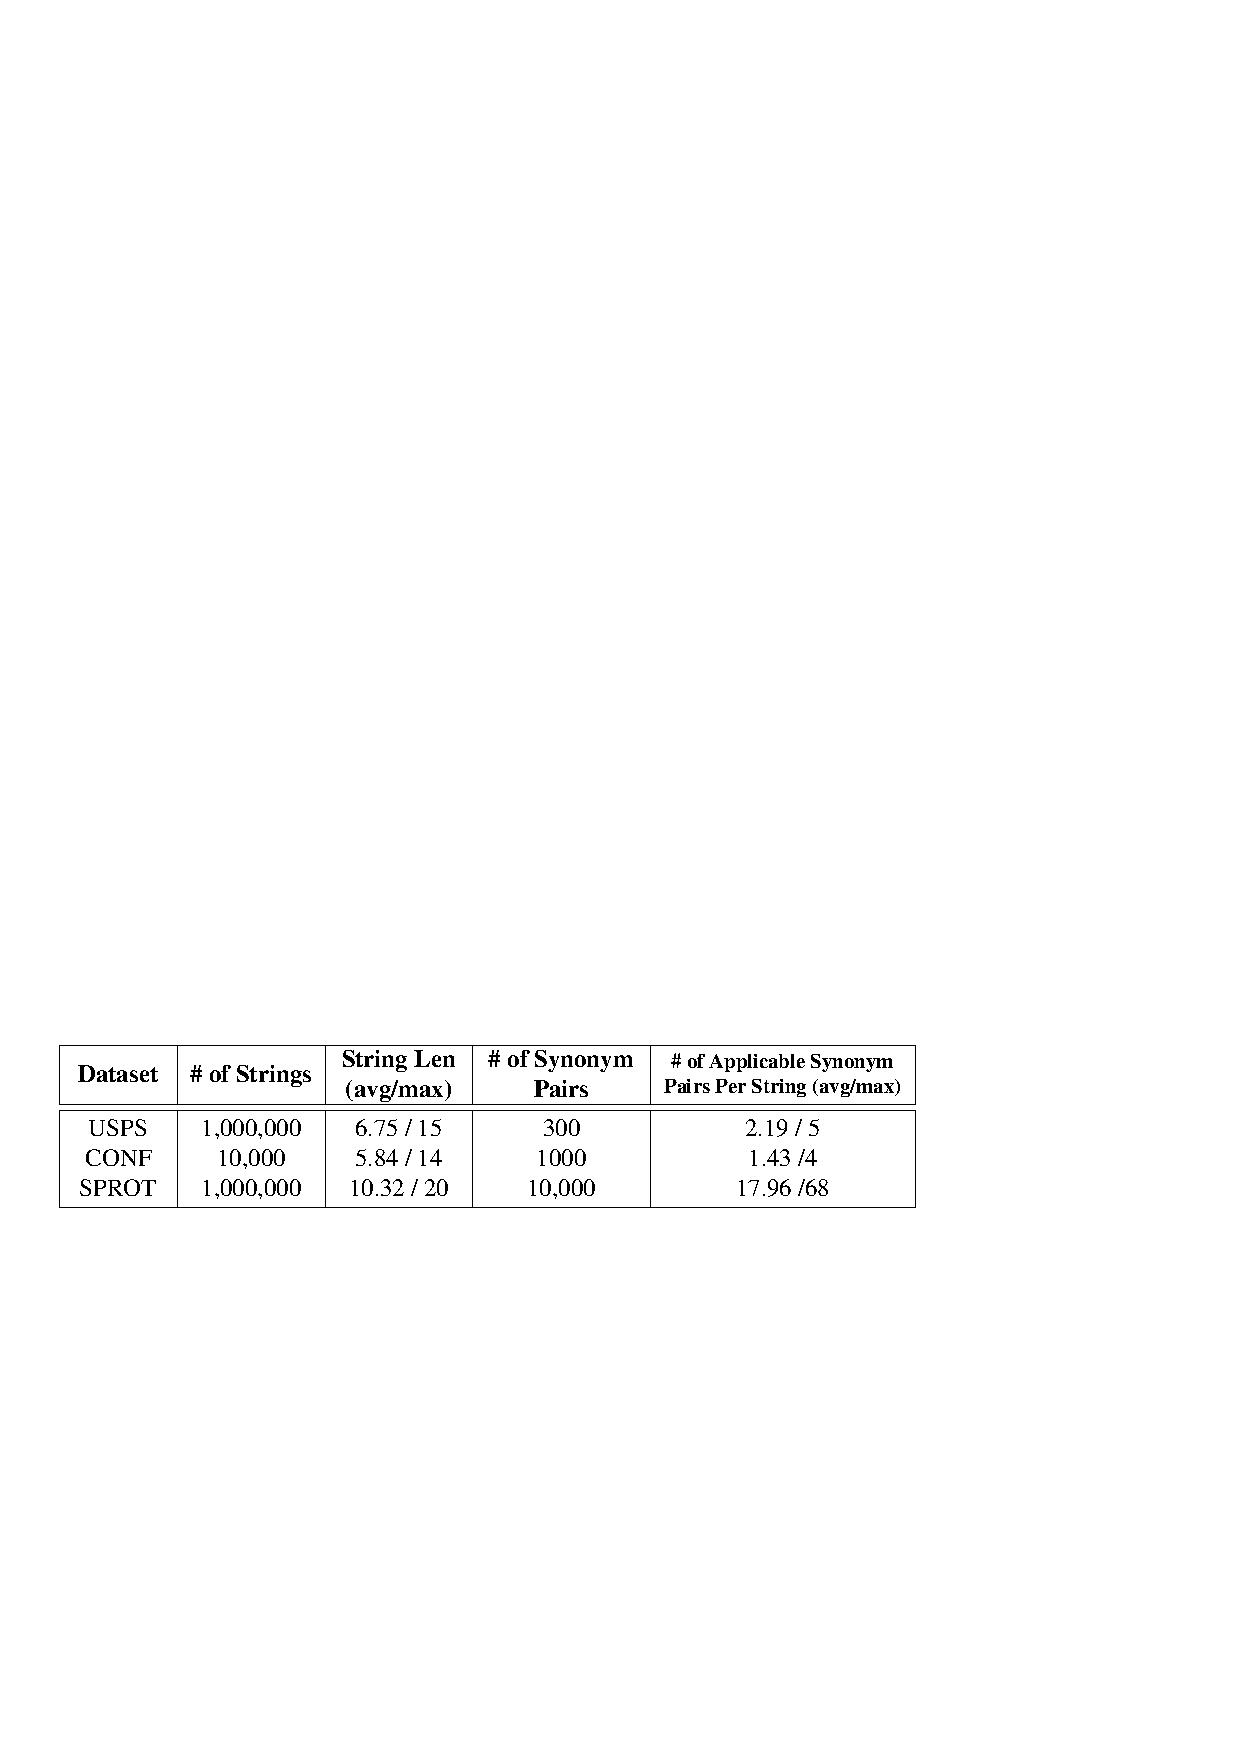
\includegraphics[width=\linewidth]{figures/Characteristics_Datasets}
   \vspace{-6mm}
  \caption{Characteristics of Datasets.}
  \label{tab:data_characteristics}
\end{figure}


Figure~\ref{tab:data_characteristics} gives the characteristics of the
three datasets.




%***************************************Conclusion and future work************************************
\section{Conclusion and future work}

We introduce a new query type, approximate string join, with taxonomy. We propose processing
models for taxonomy queries, and introduce how to build
an additional index (besides the inverted index) to support
efficient query processing. In particular, we study the problem
of how to optimize this additional index based on a
workload of queries, with the goal of minimizing query processing
cost, and propose algorithms with performance guarantees.
Our index optimization techniques are tested using
real datasets and are shown to be effective and robust.



\bibliographystyle{abbrv}
\bibliography{localrefs}



\end{document}
